\section{扩散干扰下的动力学假象}

\begin{frame}
    \frametitle{外扩散干扰下的动力学假象}

    在进行多相催化反应的动力学实验时，需要排除内、外扩散的影响，以获得反映化学现象本质的信息，如反应级数和反应活化能等。如在扩散干扰下作实验测定，将得不到这些动力学参数的本征值。

    若在处于外扩散控制的条件下进行多相催化反应的动力学实验测定，无论该反应的本征速率方程是何种形式，根据实验所得的反应速率数据与反应物浓度相关联的结果均成线性关系。这就是说处于外扩散控制区的任何反应表观上都变成了一级反应。    
    \[
        N_\mathrm{A} = k_\mathrm{G}a_\mathrm{m}(c_\mathrm{AG} - c_\mathrm{AS})
    \]
    因此，若不注意外扩散影响的排除，就有可能得出某一反应为一级反应的错误结论。特别是做实验室规模的实验测定时更应格外小心，因为实验室反应器所用的流体质量速度往往较低，从而相间传递的影响可能相当显著。

\end{frame}


\begin{frame}
    \frametitle{内扩散干扰下的动力学假象}

    外扩散阻力可以忽略时，$\alpha$级不可逆反应的反应速率可表示为
    \[
        \mathscr{R}_{\mathrm{A}}^{*}=\eta k_{\mathrm{p}} c_{\mathrm{AG}}^\alpha
    \]
    内扩散有影响的条件下，测得如下的速率方程
    \[
        \mathscr{R}_{\mathrm{A}}^{*}=k_{\mathrm{a}} c_{\mathrm{AG}}^{\alpha_\mathrm{a}}
    \]
    按理说两式是等同的，但反应级数不同，1式中的$\alpha$称为本征反应级数，而2式中的$\alpha_\mathrm{a}$则叫做表观反应级数。$\alpha$是该反应所固有的性质，是一个定值；而$\alpha_\mathrm{a}$则随内扩散影响程度的不同而改变。下面将要说明和两者之间的关系。

\end{frame}


\begin{frame}
    \frametitle{内扩散干扰下的动力学假象}

    对$\mathscr{R}_{\mathrm{A}}^{*}=\eta k_{\mathrm{p}} c_{\mathrm{AG}}^\alpha$，$\mathscr{R}_{\mathrm{A}}^{*}=k_{\mathrm{a}} c_{\mathrm{AG}}^{\alpha_\mathrm{a}}$取对数，得
    \[
        \ln \mathscr{R}_{\mathrm{A}}^{*}=\ln \eta+\ln k_{\mathrm{p}}+\alpha \ln c_{\mathrm{AG}}
    \]
    \[
        \ln \mathscr{R}_{\mathrm{A}}^{*}= \ln k_{\mathrm{a}}+\alpha_\mathrm{a} \ln c_{\mathrm{AG}}
    \]
    等温下求导，得
    \[
        \frac{\mathrm{d} \ln \mathscr{R}_{\mathrm{A}}^{*}}{\mathrm{~d} \ln c_{\mathrm{AG}}}=\alpha+\frac{\mathrm{d} \ln \eta}{\mathrm{d} \ln c_{\mathrm{AG}}}
    \]
    \[
        \mathrm{d} \ln \mathscr{R}_{\mathrm{A}}^{*} / \mathrm{d} \ln c_{\mathrm{AG}}=\alpha_{\mathrm{a}}
    \]
    两式合并后有
    \[
        \alpha_{\mathrm{a}}=\alpha+\frac{\mathrm{d} \ln \eta}{\mathrm{d} \ln c_{\mathrm{AG}}}=\alpha+\frac{\mathrm{d} \ln \eta}{\mathrm{d} \ln \phi} \frac{\mathrm{d} \ln \phi}{\mathrm{d} \ln c_{\mathrm{AG}}}
    \]

\end{frame}


\begin{frame}
    \frametitle{内扩散干扰下的动力学假象}

    若催化剂为薄片形,$\alpha$级反应的梯尔模数$\phi$为
    \[
        \phi=L \sqrt{\frac{k_{\mathrm{p}}}{2 D_{\mathrm{e}}}} \frac{c_\mathrm{AG}^{\alpha}}{\left[\int_{0}^{c_{\mathrm{AG}}} c_{\mathrm{A}}^{\alpha} \mathrm{d} c_{\mathrm{A}}\right]^{1 / 2}}=L\left[\frac{(\alpha+1) k_{\mathrm{p}}}{2 D_{\mathrm{e}}}\right]^{1 / 2} c_{\mathrm{AG}}^{(\alpha-1) / 2}
    \]
    两边取对数，然后求导得
    \[
        \mathrm{d} \ln \phi / \mathrm{d} \ln c_{\mathrm{AG}}=(\alpha-1) / 2
    \]
    那么
    \[
        \alpha_{\mathrm{a}}=\alpha+\frac{(\alpha-1)}{2} \times \frac{\mathrm{d} \ln \eta}{\mathrm{d} \ln \phi}
    \]
    

\end{frame}


\begin{frame}
    \frametitle{内扩散干扰下的动力学假象}

    \begin{itemize}
        \item 当内扩散影响不存在时$\eta =1$，        
        \[
            \alpha_{\mathrm{a}}=\alpha \qquad
        \]
        表观反应级数等于本征值。
        \item 若内扩散的影响严重，则$\eta =1/\phi$，因而有$\frac{\mathrm{d} \ln \eta}{\mathrm{d} \ln \phi} = -1$，        
        \[
            \alpha_{\mathrm{a}}= \frac{(\alpha+1)}{2}
        \]        
        本征反应级数为0、1及2时，表观反应级数分别为0.5，1及1.5。

        只有一级反应两者值相同，原因是内扩散对一级反应的影响与浓度无关。
        
        其他反应则随着内扩散干扰程度的不同，反应级数从$(\alpha+1)/2$至$\alpha$的范围内改变。
    \end{itemize}

\end{frame}


\begin{frame}
    \frametitle{内扩散对反应活化能的影响}

    设表观反应速率常数$k_\mathrm{a}$与温度的关系符合阿伦尼乌斯方程，且表观活化能为$E_\mathrm{a}$，则将$\mathscr{R}_{\mathrm{A}}^{*}=k_{\mathrm{a}} c_{\mathrm{AG}}^{\alpha_\mathrm{a}}$两边取对数，并对$1/T$求导可得
    \[
        \frac{\mathrm{d} \ln \mathscr{R}_{\mathrm{A}}^{*}}{\mathrm{~d}(1 / T)}=\frac{\mathrm{d} \ln k_{\mathrm{a}}}{\mathrm{d}(1 / T)}=-\frac{E_{\mathrm{a}}}{R}
    \]
    若本征反应速率常数$k_\mathrm{p}$与温度的关系亦可用阿伦尼乌斯方程表示，且本征活化能为$E$，则将式$\mathscr{R}_{\mathrm{A}}^{*}=\eta k_{\mathrm{p}} c_{\mathrm{AG}}^\alpha$对$1/T$求导可得
    \[
        \frac{\mathrm{d} \ln \mathscr{R}_{\mathrm{A}}^{*}}{\mathrm{~d}(1 / T)}=\frac{\mathrm{d} \ln k_{\mathrm{p}}}{\mathrm{d}(1 / T)}+\frac{\mathrm{d} \ln \eta}{\mathrm{d}(1 / T)}=\frac{-E}{R}+\frac{\mathrm{d} \ln \eta}{\mathrm{d}(1 / T)}
    \]
    两式合并并作适当改写，得
    \[
        E_{\mathrm{a}}=E-R \frac{\mathrm{d} \ln \eta}{\mathrm{d} \ln \phi} \times \frac{\mathrm{d} \ln \phi}{\mathrm{d}(1 / T)}
    \]

\end{frame}


\begin{frame}
    \frametitle{内扩散对反应活化能的影响}

    将$\alpha$级反应的梯尔模数$\phi$的表达式两边取对数，然后对$1/T$求导，忽略温度对$D_\mathrm{e}$的影响时有
    \[
        \frac{\mathrm{d} \ln \phi}{\mathrm{d}(1 / T)}=\frac{1}{2} \frac{\mathrm{d} \ln k_{\mathrm{p}}}{\mathrm{d}(1 / T)}=-\frac{E}{2 R}
    \]
    则
    \[
        E_{\mathrm{a}}=E+\frac{E}{2} \times \frac{\mathrm{d} \ln \eta}{\mathrm{d} \ln \phi}
    \]
    这便是表观活化能与本征活化能的关系式。

    表观活化能系随着内扩散干扰的程度不同而改变。
    \begin{itemize}
        \item $\phi$值甚小时，$\eta \approx 1$，此时表观活化能等于本征活化能。
        \item $\phi$值甚大时，$\frac{\mathrm{d} \ln \eta}{\mathrm{d} \ln \phi} = -1$，$E_{\mathrm{a}}=E/2$。即内扩散影响严重时，表观活化能仅为本征活化能的一半。
    \end{itemize}

\end{frame}


\begin{frame}
    \frametitle{内扩散对反应活化能的影响}

        \begin{minipage}{0.4\linewidth}
            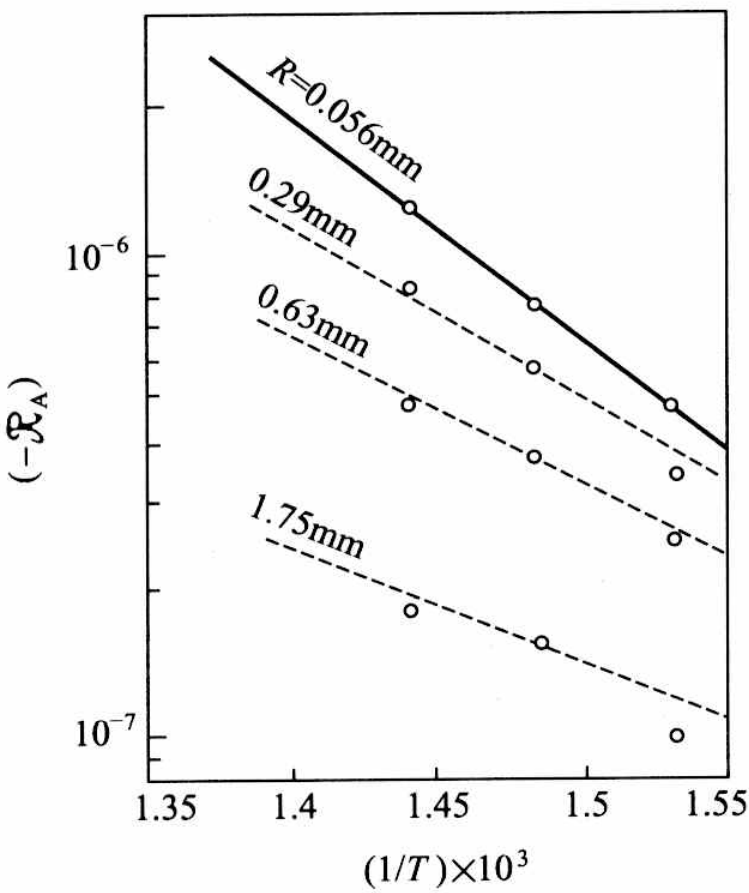
\includegraphics[width=\linewidth]{figures/fig6.10.png}
        \end{minipage}\hfill
        \begin{minipage}{0.58\linewidth}
            \begin{itemize}
                \item 由于催化剂粒度的不同，因而内扩散的影响也不相同。
                \item 对于同一粒度的实验点均能落在同一条直线上。根据直线的斜率便可确定反应活化能。
                \item 催化剂的粒度越小，直线的斜率越大。
                \item 反应的表观活化能系随催化剂粒度的增加而减小，亦即随内扩散影响的增大而减小。
            \end{itemize}
        \end{minipage}

\end{frame}


\begin{frame}
    \frametitle{扩散对多相催化反应活化能的影响}

        \begin{minipage}{0.56\linewidth}
            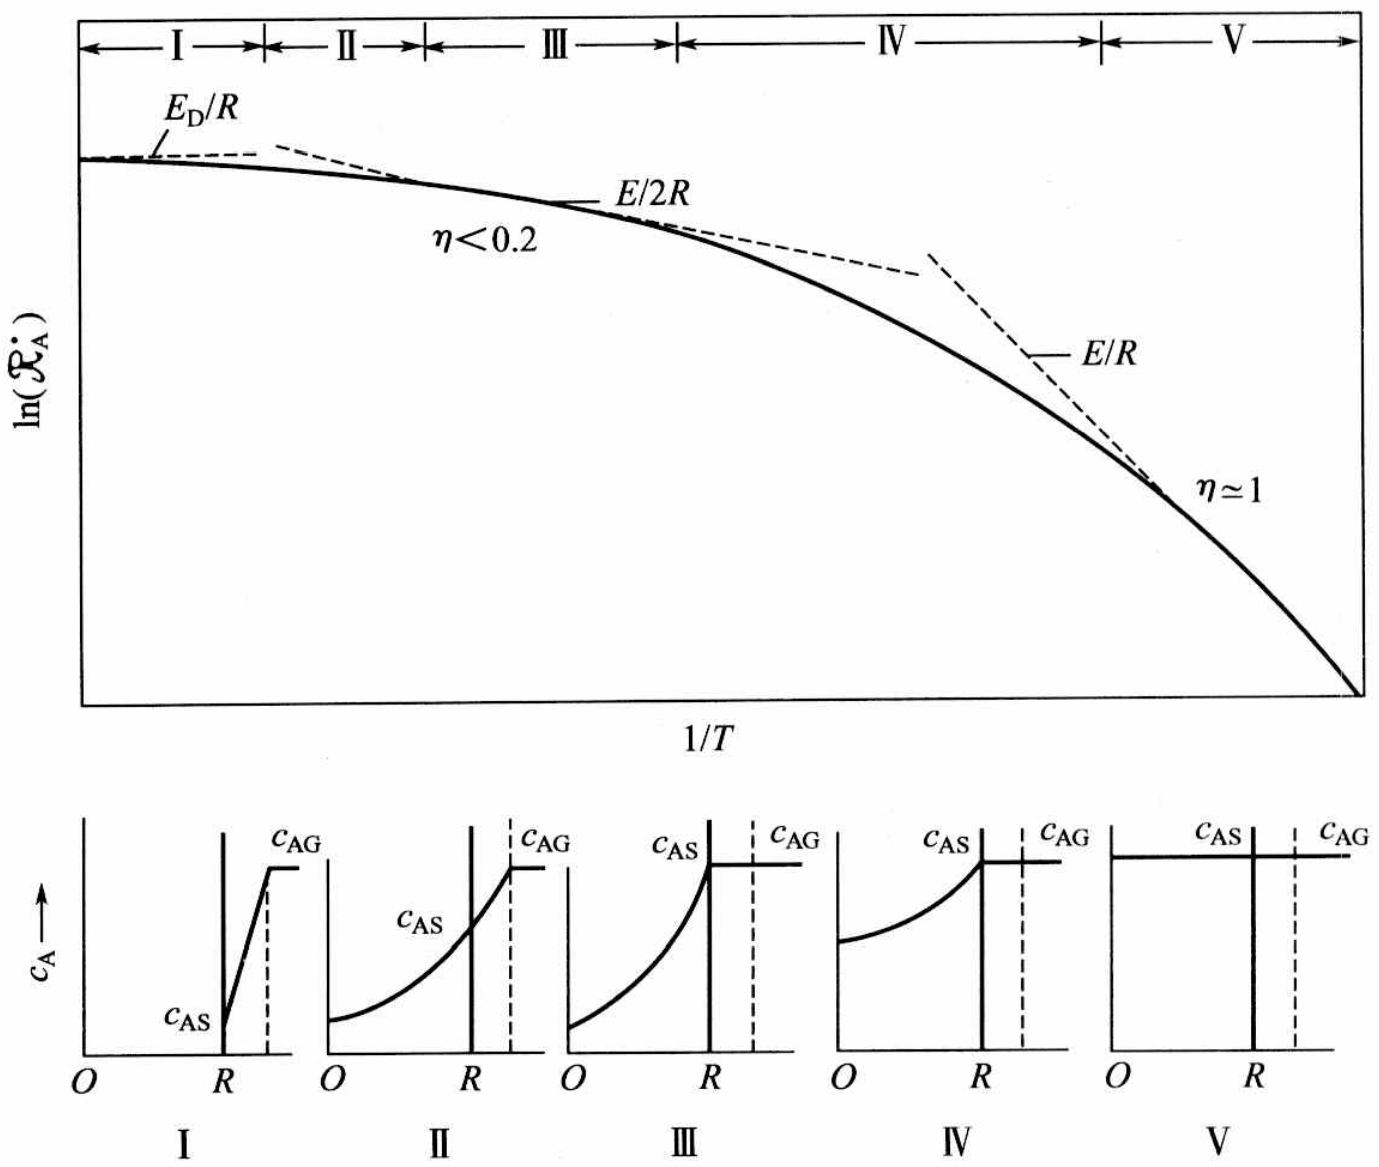
\includegraphics[width=\linewidth]{figures/fig6.11.png}
        \end{minipage}\hfill
        \begin{minipage}{0.4\linewidth}
            \begin{itemize}
                \item[I区] 高温区，外扩散控制
                
                活化能$E_\mathrm{D}$几乎为零
                \item[II区] 内外扩散过渡区
                
                活化能随温度而变
                \item[III区] 强内扩散区
                
                活化能近于常数，为$E/2$
                \item[IV区] 内扩散动力学过渡区
                
                活化能随$T$变化更显著
                \item[V区] 动力学控制区
                
                低温区，有效因子接近1
            \end{itemize}
        \end{minipage}
    

\end{frame}


\begin{frame}
    \frametitle{扩散对多相催化反应活化能的影响}

    \begin{enumerate}
        \item 多相催化反应的活化能严格说来并非定值，而是温度的函数。
        \item 只有在某些温度范围内可近似地认为是常数
            \begin{itemize}
                \item[\bullet] 外扩散控制区
                \item[\bullet] 强内扩散区
                \item[\bullet] 动力学控制区
            \end{itemize}
        \item 以上三个区的活化能值依次增高
        \item 这种差别是由于温度对化学反应和传质过程的影响不同
        \item 就一个反应而言，温度的改变会使过程从一个区转到另一个区
        \item 随着温度的降低，扩散影响趋于减弱。
    \end{enumerate}

\end{frame}